%\section{Principes de DICOM}

	\frame
	{
		\frametitle{Traduire le r\'eel en num\'erique}
		\begin{itemize}
			\item Les actions et objets du monde physique sont mod\'elis\'es de sorte \`a pouvoir les d\'ecrire et les faire exister dans le monde informatique.
			\item<2-> DICOM n'est pas la seule m\'ethode en informatique m\'edicale:
		\end{itemize}
		\begin{columns}
			\begin{column}{0.45\textwidth}
				\begin{block}<3->{DICOM}
					\begin{itemize}
						\item<4-> Mod\`eles Entit\'e / Relation: descriptions du monde r\'eel.
						\item<5-> Paire Objet-Service: un objet num\'erique.
					\end{itemize}
				\end{block}
			\end{column}
			\begin{column}{0.45\textwidth}
				\begin{block}<3->{IHE}
					\begin{itemize}
						\item<4-> Acteurs / Transactions.
						\item<6-> N'est pas limit\'e \`a l'imagerie.
						\item<7> Utilise DICOM.
					\end{itemize}
				\end{block}
			\end{column}
		\end{columns}
	}

	\frame
	{
		\frametitle{Exemple IHE: profil Scheduled Workflow (SWF.b)}
		Traduction dans le r\'eel du flux patient/examen en radiologie:
		\begin{center}
			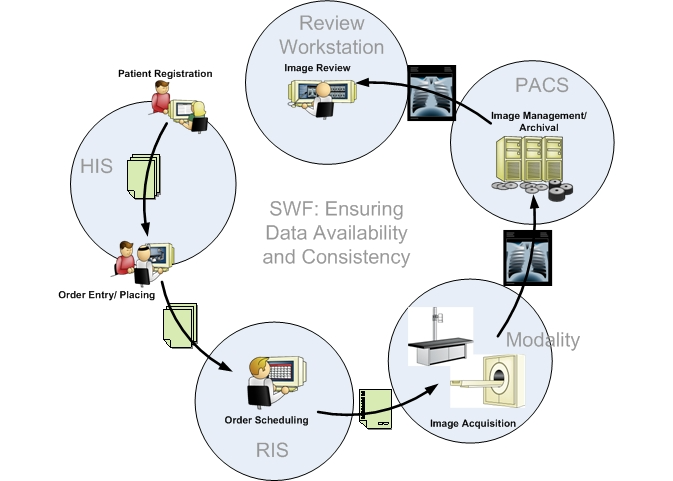
\includegraphics[width=0.8\textwidth]{../figures/SwfB-v4.png}
		\end{center}
	}

	\frame
	{
		\frametitle{Exemple DICOM: DICOM Model of the Real World}
		Traduction des relations des s\'eries d'un examen DICOM:
		\begin{center}
			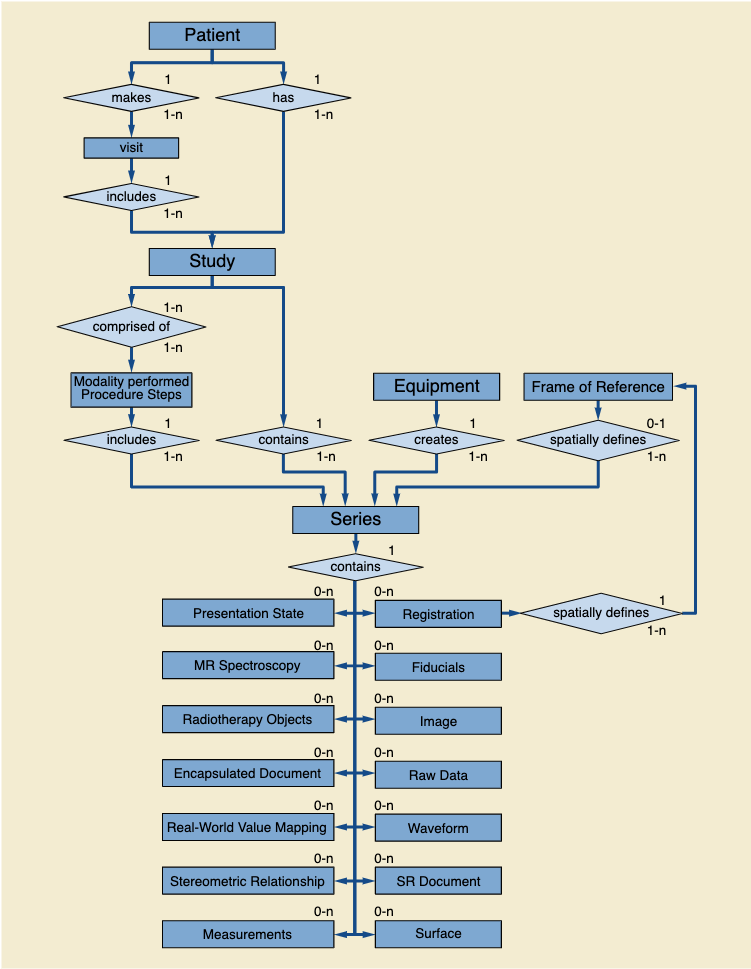
\includegraphics[scale=0.20]{../figures/PS3.png}
		\end{center}
	}
